\documentclass{article}
\usepackage[paperwidth=32cm,paperheight=18cm,margin=1cm]{geometry}
\usepackage{tikz}
\usetikzlibrary{arrows.meta,calc}
\pagestyle{empty}
\definecolor{ink}{HTML}{142D3B}
\definecolor{blue}{HTML}{78B5DC}
\definecolor{green}{HTML}{91C797}
\definecolor{gold}{HTML}{EAC977}
\definecolor{purple}{HTML}{B59AD4}
\definecolor{coral}{HTML}{DE9C88}
\tikzset{arr/.style={-{Latex[length=3mm]},very thick,draw=ink},label/.style={align=center,font=\sffamily\large,text=ink}}
% Feature volume: name, x, front width, height, depth, color, caption.
% Front face depicts spatial extent; receding depth depicts channels.
% Geometry is illustrative, not a literal scale or a count of channels.
\newcommand{\volume}[8]{%
\begin{scope}[shift={(#2,0)}]
\pgfmathsetmacro{\dx}{#5*0.65}
\pgfmathsetmacro{\dy}{#5*0.42}
\filldraw[fill=#6!55,draw=ink,line width=.7pt] (0,#4/2)--(\dx,#4/2+\dy)--(#3+\dx,#4/2+\dy)--(#3,#4/2)--cycle;
\filldraw[fill=#6!80!black,draw=ink,line width=.7pt] (#3,-#4/2)--(#3+\dx,-#4/2+\dy)--(#3+\dx,#4/2+\dy)--(#3,#4/2)--cycle;
\foreach \t in {.2,.4,.6,.8}{\draw[ink!35,line width=.3pt] (#3+\t*\dx,-#4/2+\t*\dy)--(#3+\t*\dx,#4/2+\t*\dy);}
\filldraw[fill=#6,draw=ink,line width=.8pt] (0,-#4/2) rectangle (#3,#4/2);
\coordinate (#1-in) at (0,0);
\coordinate (#1-out) at (#3+\dx,0);
\node[label,font=\sffamily\bfseries\large] at (#3/2,3.5) {#7};
\node[label] at (#3/2,-3.0) {#8};
\end{scope}}
\newcommand{\heading}[2]{\begin{center}{\Huge\sffamily\bfseries\color{ink}#1}\par\vspace{.25cm}{\large\sffamily\color{ink}#2}\end{center}\vspace{.6cm}}
\begin{document}
\heading{Custom ResNet + MixUp}{3D feature volumes through the network}
\begin{center}
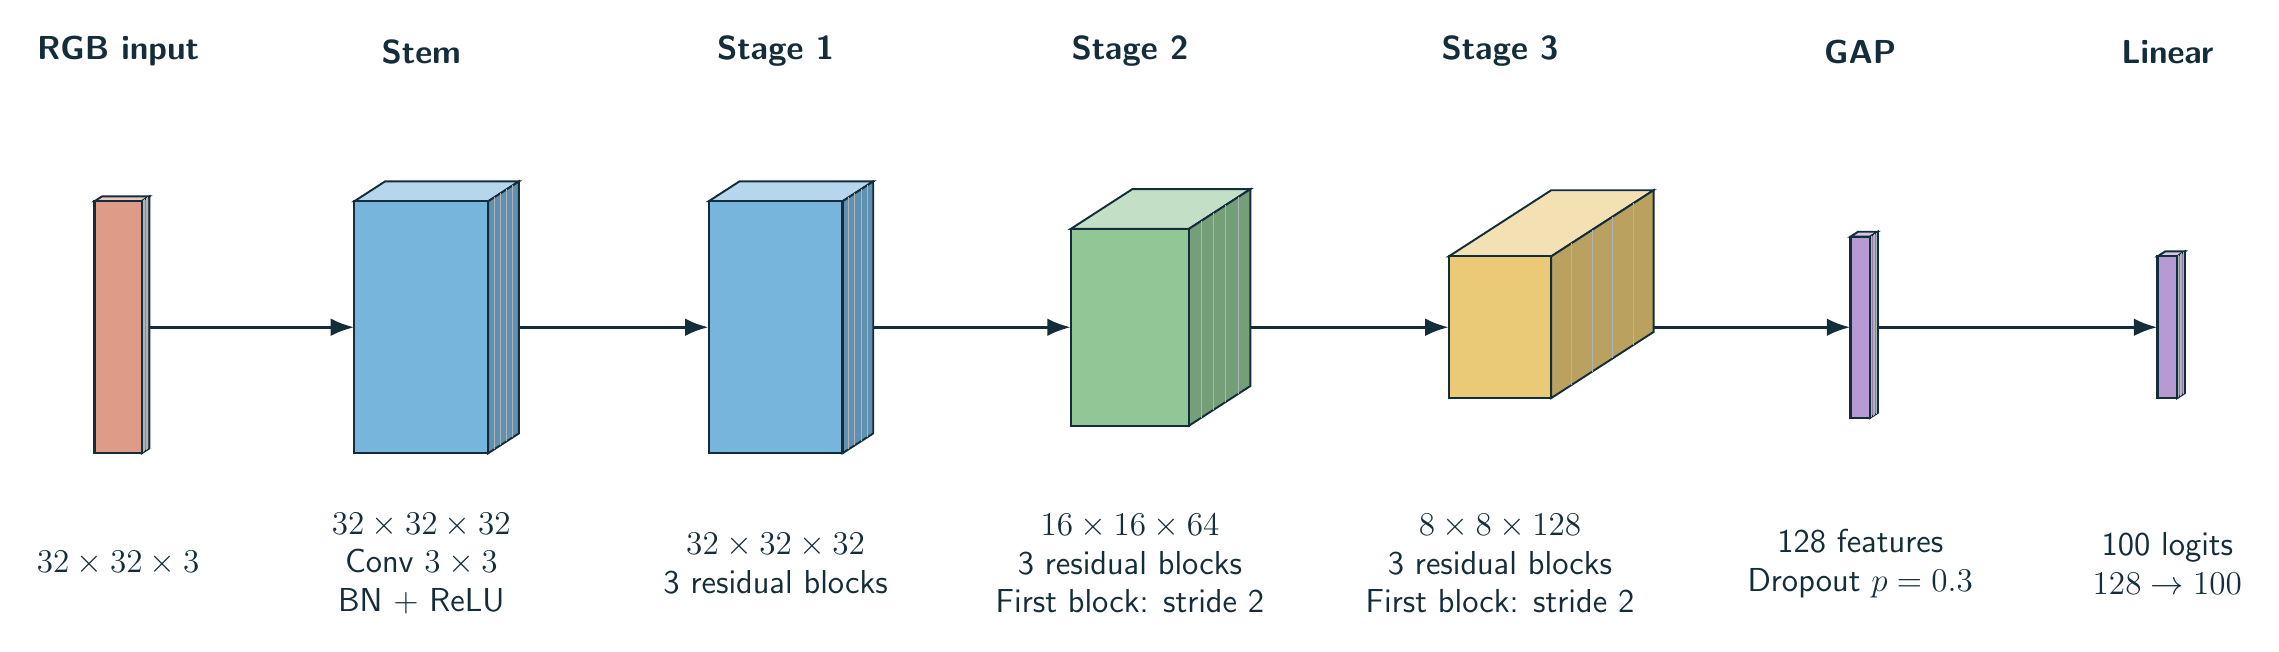
\begin{tikzpicture}
\volume{input}{0}{.6}{3.2}{.15}{coral}{RGB input}{$32\times32\times3$}
\volume{stem}{3.3}{1.7}{3.2}{.6}{blue}{Stem}{$32\times32\times32$\\Conv $3\times3$\\BN + ReLU}
\volume{s1}{7.8}{1.7}{3.2}{.6}{blue}{Stage 1}{$32\times32\times32$\\3 residual blocks}
\volume{s2}{12.4}{1.5}{2.5}{1.2}{green}{Stage 2}{$16\times16\times64$\\3 residual blocks\\First block: stride 2}
\volume{s3}{17.2}{1.3}{1.8}{2.0}{gold}{Stage 3}{$8\times8\times128$\\3 residual blocks\\First block: stride 2}
\volume{gap}{22.3}{.25}{2.3}{.15}{purple}{GAP}{128 features\\Dropout $p=0.3$}
\volume{fc}{26.2}{.25}{1.8}{.15}{purple}{Linear}{100 logits\\$128\to100$}
\foreach \a/\b in {input/stem,stem/s1,s1/s2,s2/s3,s3/gap,gap/fc}{\draw[arr] (\a-out)--(\b-in);}
\end{tikzpicture}\par\vspace{1.2cm}
{\large\sffamily Front face: spatial dimensions. Depth: channel dimension. Shapes are not to scale.}\par\vspace{.25cm}
{\large\sffamily 1,096,196 parameters. MixUp is a training augmentation, not a network layer.}
\end{center}
\newpage
\heading{Residual block in 3D}{Two convolution layers with a shortcut connection}
\begin{center}
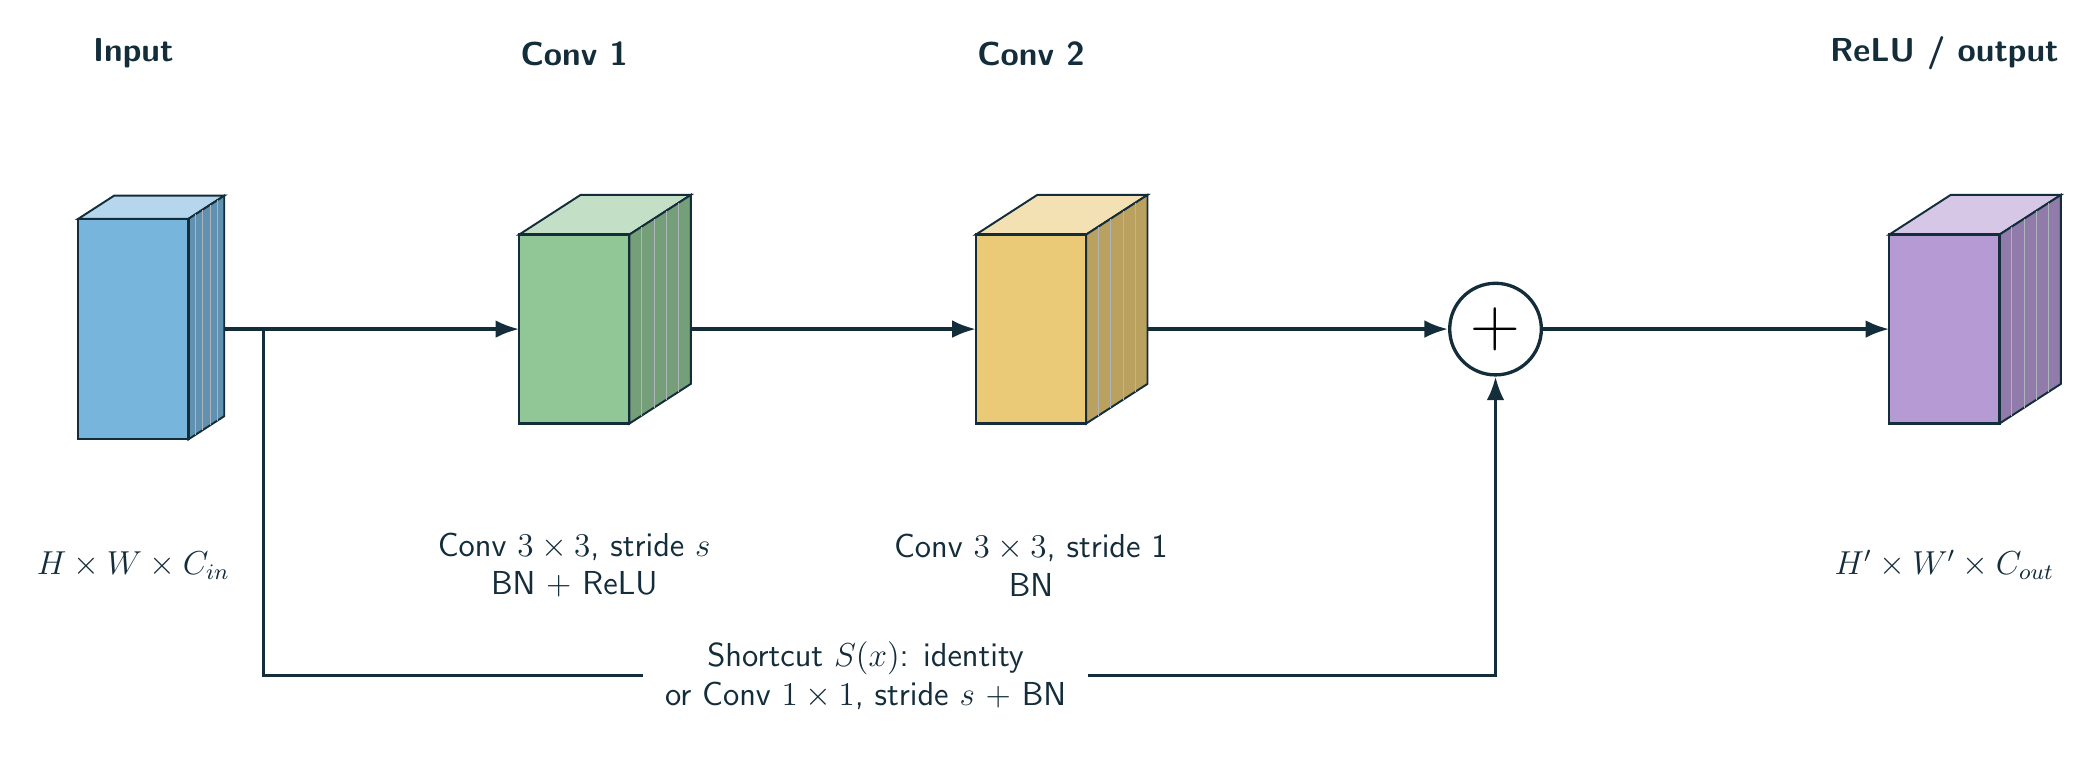
\begin{tikzpicture}
\volume{x}{0}{1.4}{2.8}{.7}{blue}{Input}{$H\times W\times C_{in}$}
\volume{c1}{5.6}{1.4}{2.4}{1.2}{green}{Conv 1}{Conv $3\times3$, stride $s$\\BN + ReLU}
\volume{c2}{11.4}{1.4}{2.4}{1.2}{gold}{Conv 2}{Conv $3\times3$, stride 1\\BN}
\node[draw=ink,circle,very thick,minimum size=1cm,font=\Huge] (sum) at (18,0) {$+$};
\volume{out}{23}{1.4}{2.4}{1.2}{purple}{ReLU / output}{$H'\times W'\times C_{out}$}
\draw[arr](x-out)--(c1-in);\draw[arr](c1-out)--(c2-in);\draw[arr](c2-out)--(sum);\draw[arr](sum)--(out-in);
\draw[arr] ($(x-out)+(.5,0)$)--++(0,-4.4)-| (sum.south);
\node[label,fill=white,inner sep=8pt] at (10,-4.4) {Shortcut $S(x)$: identity\\or Conv $1\times1$, stride $s$ + BN};
\end{tikzpicture}\par\vspace{.6cm}
{\Large\sffamily $y=\mathrm{ReLU}\bigl(F(x)+S(x)\bigr)$}\par\vspace{.3cm}
{\large\sffamily Both branches have matching output dimensions. Volumes are illustrative.}
\end{center}
\newpage
\heading{Swin-T pretrained on ImageNet-1K}{Hierarchical feature volumes and a new 100-class head}
\begin{center}
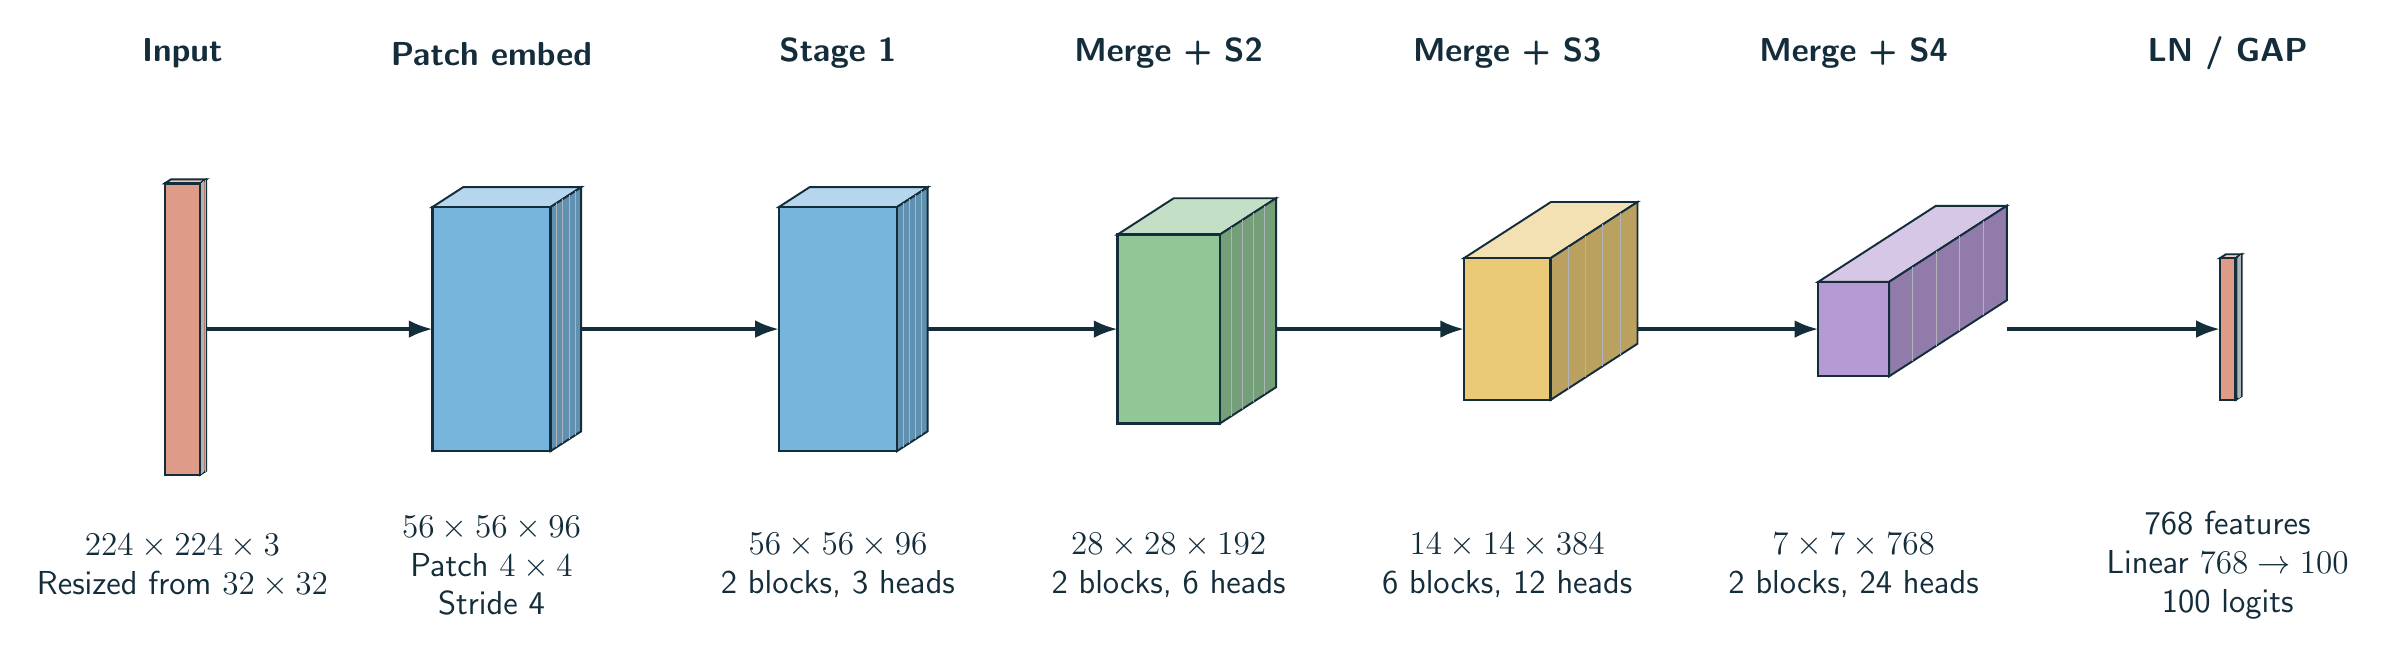
\begin{tikzpicture}
\volume{im}{0}{.45}{3.7}{.12}{coral}{Input}{$224\times224\times3$\\Resized from $32\times32$}
\volume{p}{3.4}{1.5}{3.1}{.6}{blue}{Patch embed}{$56\times56\times96$\\Patch $4\times4$\\Stride 4}
\volume{a}{7.8}{1.5}{3.1}{.6}{blue}{Stage 1}{$56\times56\times96$\\2 blocks, 3 heads}
\volume{b}{12.1}{1.3}{2.4}{1.1}{green}{Merge + S2}{$28\times28\times192$\\2 blocks, 6 heads}
\volume{c}{16.5}{1.1}{1.8}{1.7}{gold}{Merge + S3}{$14\times14\times384$\\6 blocks, 12 heads}
\volume{d}{21.0}{.9}{1.2}{2.3}{purple}{Merge + S4}{$7\times7\times768$\\2 blocks, 24 heads}
\volume{head}{26.1}{.2}{1.8}{.12}{coral}{LN / GAP}{768 features\\Linear $768\to100$\\100 logits}
\foreach \a/\b in {im/p,p/a,a/b,b/c,c/d,d/head}{\draw[arr](\a-out)--(\b-in);}
\end{tikzpicture}\par\vspace{1.2cm}
{\large\sffamily Each stage alternates window and shifted-window attention, with $7\times7$ windows.}\par\vspace{.25cm}
{\large\sffamily Patch merging halves spatial size and doubles channels. Volumes are not to scale.}\par\vspace{.25cm}
{\large\sffamily 27,596,254 parameters after replacing the original classifier.}
\end{center}
\end{document}
